\documentclass[12pt]{article}
%\usepackage{graphicx}
\usepackage[pdftex]{graphicx}
\usepackage{fancyhdr}
\usepackage[latin1]{inputenc}
\usepackage{moreverb}
\usepackage{amssymb}
%\usepackage[sectionbib]{natbib}
\usepackage[english]{babel}
\pagestyle{fancy}
\begin{document}


\fancyhead[LE,LO]{
\includegraphics[height=13pt]{molflow.png}}
\fancyhead[CE,CO]{}
\fancyhead[RE,RO]{\bfseries\nouppercase\leftmark}
\fancyfoot[LO,LE]{}
\fancyfoot[RO,RE]{}
\fancyfoot[CO,CE]{}
\renewcommand{\footrulewidth}{0.4pt}
\renewcommand{\headrulewidth}{0.4pt}

\title{A level0 to level1b database for Odin-SMR\\
       \vspace*{85mm}}
\author{
	Joakim M\"{o}ller, joakim.moller@molflow.com\\
        Bengt Rydberg, bengt.rydberg@molflow.com\\
        %Dept. of Geo and Space Sciences\\%\vspace*{10mm}
        %Chalmers University of Technology\\
        Gothenburg, Sweden\\
        }
%\date{Gothenburg, Sweden}

\begin{titlepage}
	    
\includegraphics[width=0.3\textwidth]{molflow.png}
  \begin{flushright}
    \noindent\rule{\textwidth}{2pt}
    \vspace{1cm}
    \begin{huge}
	   A level0 to level1b database for Odin-SMR\\
    \end{huge}
      \vspace{1cm}
    \today\\
    \noindent\rule{\textwidth}{2pt}
    \vspace{1cm}\\
    \begin{minipage}[t]{0.3\textwidth}
    \end{minipage}%
    \begin{minipage}[t]{0.30\textwidth}
	Joakim M\"{o}ller\\
        Bengt Rydberg
    \end{minipage}%
    \begin{minipage}[t]{0.4\textwidth}
      \begin{flushright}
        joakim.moller@molflow.com
	bengt.rydberg@molflow.com
      \end{flushright}
\end{minipage}
  \vspace{8cm}
\end{flushright}
\end{titlepage}

%\thispagestyle{empty}
%\newpage
\tableofcontents
\thispagestyle{empty}
\newpage
\setcounter{page}{1}
\section{Overview}
The aim of this project has been to make the existing
calibration procedure, i.e. the processing of various
level0 files to calibrated spectra, of Odin-SMR data 
more transparent.
A database with tables for level0-, level1a-, and level1b data,
and data import scripts have been developed (see Fig.~\ref{fig:database}).

The old calibration code has to a very large extend been re-used,
but the code has been partitioned into several smaller scripts,
that stores data into database tables. This will not only make
further development more simple, the processing can be significant more
time efficient as well. For example, if one wants to test a new
calibration version (level1a to level1b) one does not have to
re-process all data below level1b.       

This document describes: \\
-- the database and how to import 
data into the various database tables\\
-- calibration scheme\\
-- required packages and installations\\

\clearpage
\newpage




\section{The Database}
\subsection{Overview}
\begin{figure}[!t]
\centering
%\includegraphics[scale=0.7]{odingraph3.png}
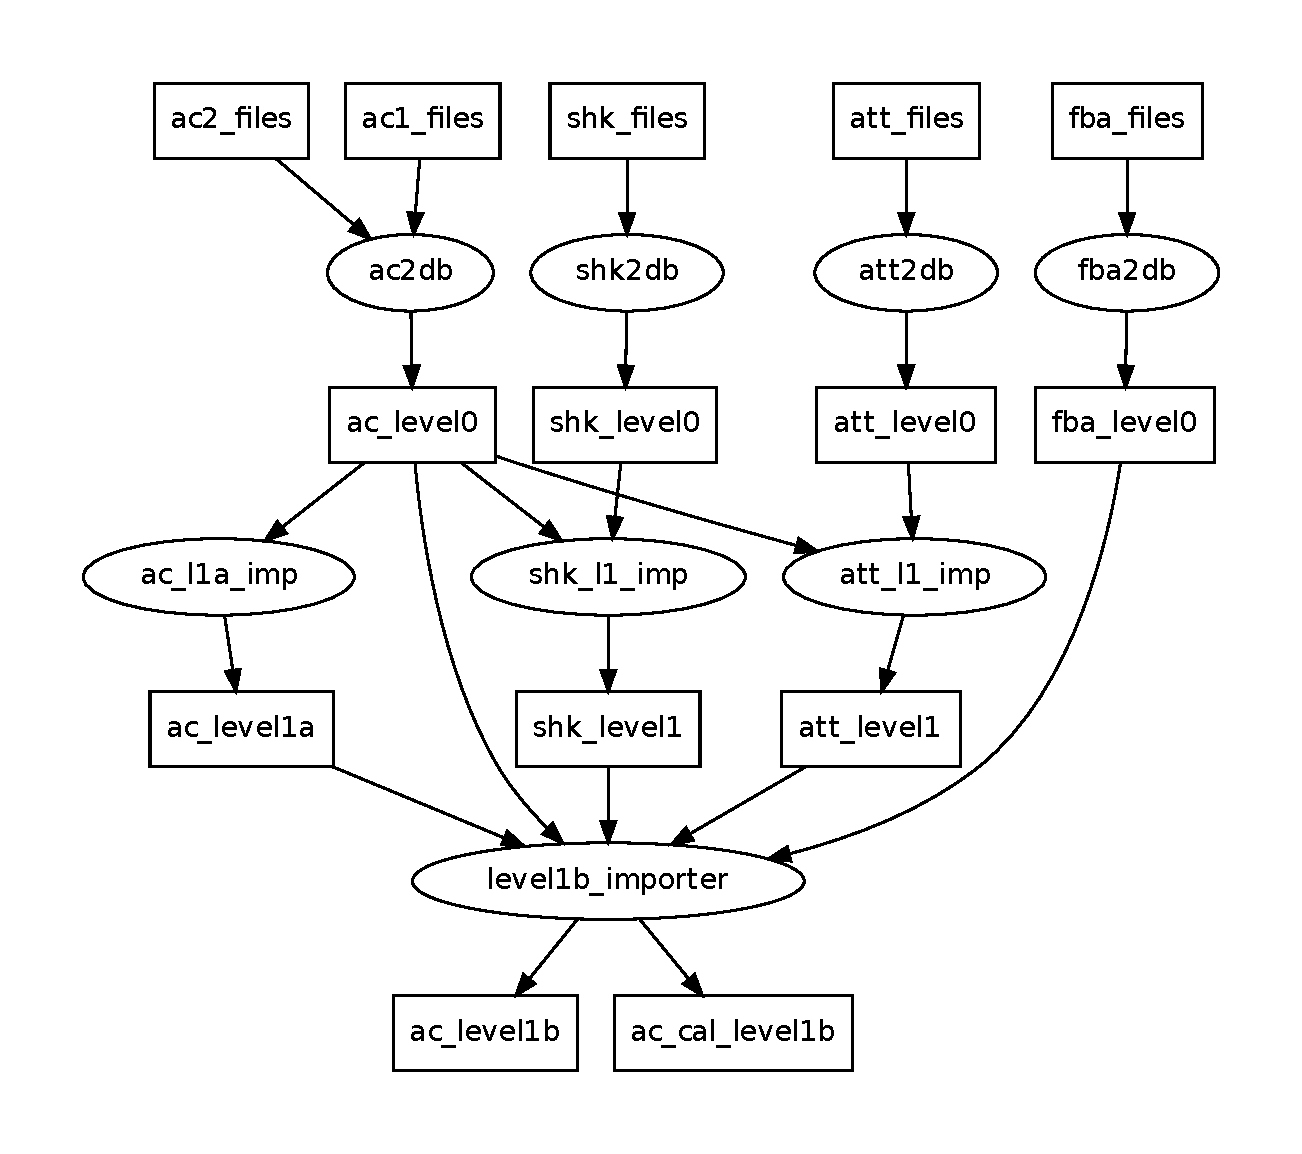
\includegraphics[scale=0.7]{dataflow.pdf}
\caption{A dependency diagram of the processing and database system. 
The top layer represents level0 files.
The names in the ovals represent executables that process and import
data into database tables (named in the boxes below the top layer).
The graph can be interpreted in the following way: 
att\underline{ }l1\underline{ }imp search for data
in the att\underline{ }level0 and ac\underline{ }level0 
database tables in order to ultimately import data into the
att\underline{ }level1 table, but is independent of all
other processes in the figure.In the remaining text
att\underline{ }l1\underline{ }imp= attitude\underline{ }level1\underline{ }importer, shk\underline{ }l1\underline{ }imp=shk\underline{ }level1\underline{ }importer, and ac\underline{ }l1a\underline{ }imp= ac\underline{ }level1a\underline{ }importer
}
\label{fig:database}
\end{figure}


The database consists of nine tables (see Fig.~\ref{fig:database}):\\ 
%which can be categorized into different levels:\\
-- four level0 tables (ac\underline{ }level0, attitude\underline{ }level0, 
shk\underline{ }level0 [housekeeping], and fba\underline{ }level0 
[reference signal type]
) that contains data from level0 files,\\
-- three level1 or level1a (attitude\underline{ }level1, shk\underline{ }level1,
ac\underline{ }level1a) that contains processed level0 data,\\ 
-- two level1b tables (ac\underline{ }level1b that contains calibrated 
spectrum towards target and
ac\underline{ }cal\underline{ }level1b that contains   
sideband ratio spectrum and calibration spectrum)

To clarify the different levels in terms of auto-correlator (ac) data:\\
-- ac\underline{ }level0 contains the measured correlation
coefficients (normalised by integration time)\\
-- ac\underline{ }level1a contains spectrum in the frequency domain\\
-- ac\underline{ }level1b contains intensity (and frequency) calibrated spectrum


\subsection{Level0 tables}
Four level0 tables: ac\underline{ }level0, attitude\underline{ }level0, 
shk\underline{ }level0, and fba\underline{ }level0 contains 
data from level0 files, and the tables are here described in 
some more details. 
ac2db, att2db, shk2db, and fba2db are executables responsible for importing
data into these tables (how to import data can be seen
Sect.~\ref{sec:import}).
Satellite time word (stw) is a key-column in all these tables.
However, data in the different level0 files come on different 
stw resolution. Only the stw in fba\underline{ }level0
matches with the stw in ac\underline{ }level0 (see Appendix
how fba\underline{ }level0 and ac\underline{ }level0 matches).
  
All the level0 tables, except fba\underline{ }level0, has a higher
level (level1) table, where stw matches with ac\underline{ }level0. 
Thus, it is simple to match level1 data and ac\underline{ }level0
using stw in SQL queries, but other level0 data does not match.


%attitude\underline{ }level0
%contains attitude data, shk\underline{ }level0 contains housekeeping
%data.
  


\clearpage
\newpage
\subsubsection*{Table columns}

\begin{table}[ht]
\caption{ac\underline{ }level0}
\centering
\begin{tabular}{l l l}
\hline\hline
Column & Type & Description \\ [0.5ex]
\hline
stw (key)            & bigint                                &  - \\
backend (key)        & ('AC1','AC2')                         & -\\
frontend             & ('549','495','572','555','SPL','119') & -\\
sig\underline{ }type & ('REF','SIG')                         & -\\
ssb\underline{ }att  & integer[]                             & -\\
ssb\underline{ }fq   & integer[]                             & the four lo freq. of the ssb modules\\
prescaler            & integer                               & -\\
inttime              & real                                  & -\\
mode                 & integer                               & correlator configuration\\
acd\underline{ }mon  & bytea, shape=(8,2),dtype='float64'    & monitor data\\
cc                   & bytea, shape=(8,96),dtype='float64'   & correlation coefficients\\[1ex]
\hline
\end{tabular}
\label{table:ac0}
\end{table}
How to extract column data that has Type bytea and integer[] using
python can be seen in the Appendix.
\begin{table}[ht]
\caption{fba\underline{ }level0, to be used together with ac\underline{ }level0
to find out what sig\underline{ }type 'REF' means}
\centering
\begin{tabular}{l l l}
\hline\hline
Column & Type & Description \\ [0.5ex]
\hline
stw (key) & bigint & - \\
mech\underline{ }type & ('SK1','SK2','CAL') & -\\[1ex]
\hline
\end{tabular}
\label{table:fba0}
\end{table}

%\subsubsection{attitude\underline{ }level0} 
%\subsubsection{attitude\underline{ }level0}
\begin{table}[ht]
\caption{attitude\underline{ }level0}
\centering
\begin{tabular}{l l l}
\hline\hline
Column & Type & Description \\ [0.5ex]
\hline
stw (key) & bigint             & - \\
soda (key) & integer             & - \\
year     & integer            & -\\
mon     & integer            & -\\
day     & integer            & -\\
hour    & integer            & -\\
min     & integer            & -\\
secs    & double precision   & -\\
orbit   & double precision   & -\\ 
qt      & double precision[] & qtarget (4-vector)\\
qa      & double precision[] & qachieved (4-vector)\\
qe      & double precision[] & qerror (3-vector)\\
gps     & double precision[] & gps position and velocity (6-vector)\\
acs     & double precision   & -\\[1ex]
\hline
\end{tabular}
\label{table:att0}
\end{table}



%\subsubsection{shk\underline{ }level0}
\begin{table}[ht]
\caption{shk\underline{ }level0}
\centering
\begin{tabular}{l l l}
\hline\hline
Column & Type & Description \\ [0.5ex]
\hline
stw (key) & bigint & - \\
shk\underline{ }type (key) & ('LO495','LO549','LO555','LO572',  & lo freq.\\
 & 'SSB495','SSB549','SSB555','SSB572', & ssb tunings\\
 & 'mixC495','mixC549','mixC555','mixC572', & mixer current\\
 & 'imageloadA','imageloadB','hotloadA','hotloadB' & temperatures\\  
 & 'mixerA','mixerB','lnaA','lnaB' &  temperatures\\ 
 & '119mixerA','119mixerB','warmifA','warmifB') & temperatures  \\
shk\underline{ }value & real & -\\[1ex]
\hline
\end{tabular}
\label{table:shk0}
\end{table}


\clearpage
\newpage

\subsection{Level1 and level1a tables}
attitude\underline{ }level1, shk\underline{ }level1, and
ac\underline{ }level1a contains processed level0 data.
attitude\underline{ }level1\underline{ }importer,
ac\underline{ }level1a\underline{ }importer,
and shk\underline{ }level1\underline{ }importer
are responsible for importing data into these tables.
stw and backend are key-columns in these tables,
and these key-columns matches among these tables.


\subsubsection*{Table columns}

\begin{table}[ht]
\caption{attitude\underline{ }level1}
\centering
\begin{tabular}{l l l}
\hline\hline
Column & Type & Description \\ [0.5ex]
\hline
 stw (key)  & bigint             & - \\
 backend (key) & ('AC1','AC2')   & - \\
 soda (key) & integer            & - \\
 mjd        & double precision   & - \\  
 lst        & real               & - \\   
 orbit      & double precision   & - \\   
 latitude   & real               & - \\    
 longitude  & real               & - \\    
 altitude   & real               & - \\    
 skybeamhit & integer            & - \\    
 ra2000     & real               & - \\    
 dec2000    & real               & - \\    
 vsource    & real               & - \\    
 qtarget    & double precision[] & - \\ 
 qachieved  & double precision[] & - \\ 
 qerror     & double precision[] & - \\ 
 gpspos     & double precision[] & - \\    
 gpsvel     & double precision[] & - \\  
 sunpos     & double precision[] & - \\  
 moonpos    & double precision[] & - \\  
 sunzd      & real               & - \\  
 vgeo       & real               & - \\ 
 vlsr       & real               & - \\ 
 alevel     & integer            & -\\[1ex]
\hline
\end{tabular}
\label{table:att1}
\end{table}


   
%%%%%%%%%%
\begin{table}[ht]
\caption{shk\underline{ }level1}
\centering
\begin{tabular}{l l l}
\hline\hline
Column & Type & Description \\ [0.5ex]
\hline
 stw (key)       & bigint           & - \\
 backend (key)   & ('AC1','AC2')    & -\\ 
 frontendsplit & ('549','495','572','555','SPL','119') & -\\
 lo         & real             & -\\ 
 ssb        & real             & -\\ 
 mixc       & real             & -\\  
 imageloada & real             & -\\
 imageloadb & real             & -\\
 hotloada   & real             & -\\ 
 hotloadb   & real             & -\\
 mixera     & real             & -\\
 mixerb     & real             & -\\
 lnaa       & real             & -\\
 lnab       & real             & -\\
 mixer119a  & real             & -\\
 mixer119b  & real             & -\\
 warmifa    & real             & -\\
 warmifb    & real             & -\\[1ex]
\hline
\end{tabular}
\label{table:shk1}
\end{table}


\begin{table}[ht]
\caption{ac\underline{ }level1a}
\centering
\begin{tabular}{l l l}
\hline\hline
Column & Type & Description \\ [0.5ex]
\hline
stw (key)    & bigint         & - \\
backend (key) & ('AC1','AC2')  & -\\
spectra & bytea, shape=(112*8,),dtype='float64' & spectrum in the \\
& & frequency domain\\[1ex]
\hline
\end{tabular}
\label{table:ac1a}
\end{table}

\clearpage
\newpage

\subsection{Level1b tables}
ac\underline{ }level1b contains calibrated target spectra
and also calibrated reference spectra.
ac\underline{ }cal\underline{ }level1b contains sideband ratio 
spectrum and calibration (tsys) spectrum.
Level1b\underline{ }importer (further described in
Sect.~\ref{sec:cal}) is responsible for
importing data into these tables.

\subsubsection*{Table columns}

\begin{table}[ht]
\caption{ac\underline{ }level1b}
\centering
\begin{tabular}{l l l}
\hline\hline
Column & Type & Description \\ [0.5ex]
\hline
 stw (key)               & bigint           & - \\
 backend (key)           & ('AC1','AC2')    & -\\
 version (key)            & integer          & -\\         
 intmode (key)           & integer          & -\\
 soda (key)           & integer          & -\\
 spectra            & bytea,shape=(channels,),dtype='float64' & calibrated spectrum\\       
 channels           & integer          & -\\          
 skyfreq            & double precision & -\\ 
 lofreq             & double precision & -\\ 
 restfreq           & double precision & -\\ 
 maxsuppression     & double precision & -\\ 
 tsys               & real             & -\\ 
 sourcemode         & ('STRAT','ODD\underline{ }H','ODD\underline{ }N', & -\\
 & 'WATER','SUMMER','DYNAM') & \\ 
 freqmode           & integer          & -\\ 
 efftime            & real             & -\\ 
 sbpath             & real             & -\\ 
 calstw             & bigint           & stw of calibration spectrum\\[1ex]
\hline
\end{tabular}
\label{table:ac1a}
\end{table}


\begin{table}[ht]
\caption{ac\underline{ }cal\underline{ }level1b}
\centering
\begin{tabular}{l l l}
\hline\hline
Column & Type & Description \\ [0.5ex]
\hline
 stw (key)           & bigint            &- \\
 backend (key)       & ('AC1','AC2')     & -\\
 version (key)       & integer           & -\\
 spectype (key)      & ('CAL','SSB')         & -\\
 intmode (key)       & integer           & -\\
 soda (key)       & integer           & -\\
 spectra        & bytea             & shape=(channels,),dtype='float64'\\
 channels       & integer           & -\\
 skyfreq        & double precision  & -\\
 lofreq         & double precision  & -\\
 restfreq       & double precision  & -\\
 maxsuppression & double precision  & -\\
 sourcemode     & ('STRAT','ODD\underline{ }H','ODD\underline{ }N', & -\\
& 'WATER','SUMMER','DYNAM','N/A')   & \\
 freqmode       & integer           & -\\ 
 sbpath         & real              &\\
 tspill         & real              &\\[1ex]
\hline
\end{tabular}
\label{table:ac1a}
\end{table}

\clearpage
\newpage

\subsection{Importing data}
\label{sec:import}
Importing all data from level0 files into the level0 tables are done 
by the following commands:
\begin{verbatim}
$bin/ac2db /home/bengt/Downloads/02f8deef.ac1
$bin/ac2db /home/bengt/Downloads/02f8deef.ac2
$bin/att2db /home/bengt/Downloads/02f8a74e.att
$bin/shk2db /home/bengt/Downloads/02f8def1.shk
$bin/fba2db /home/bengt/Downloads/02f8def0.fba
\end{verbatim}
Importing data into the three first level1 tables are done 
with the following commands:
\begin{verbatim}
$bin/shk_level1_importer
$bin/att_level1_importer 17
$bin/ac_level1a_importer
\end{verbatim}
where the argument 17 means that only attitude data from soda version
17 will be considered by the import script. All data that is available will 
be imported into the different tables 

The calibration of ac\underline{ }level1a data is then done by:
\begin{verbatim}
$bin/level1b_importer orbit backend
e.g.
$bin/level1b_importer 8575 AC1
\end{verbatim}
using the old calibration scheme, or
\begin{verbatim}
$bin/level1b_window_importer orbitstart orbitend backend soda filter
e.g.
$bin/level1b_window_importer 8575 8577 AC1 17 1
\end{verbatim}
using an updated calibration scheme (Sect.~\ref{sec:cal}).
Scans from AC1 that start within orbit 8575 to 8577 will be calibrated,    
and resulting data will be inserted in table ac\underline{ }level1b 
(calibrated spectra) and
ac\underline{ }cal\underline{ }level1b (tsys and ssb spectra). 
%The old calibration procedure is performed based on data from
%one orbit, but ac\underline{ }cal\underline{ }level1b
%uses data from all scans that starts in an orbit.
%This means that there is a difference in which data
%that is considered in both the start and the end of the orbit
%(this is very easy to change). 
level1b\underline{ }window\underline{ }importer assumes that all data 
from the orbits
is imported into the database, but nothing is clearly done if not
enough data is found.
 
Extracting calibrated spectrum and data (in a similiar structure as 
the official level1b files)
from the database into a hdf5 format
file can be done by:
\begin{verbatim}
$bin/level1b_exporter orbit backend outputfile.hdf5
\end{verbatim}

\section{Calibration procedure}
\label{sec:cal}

\subsection{ac\underline{ }level0 to ac\underline{ }level1a}
The processing of ac\underline{ }level0 data
(measured modified correlation coefficients)
to ac\underline{ }level1a (spectrum in the frequency domain)
is partly described in \cite{notes}, and is in short given here :\\
-- correlation coefficients from the eight correlator chips
with 96 lags each are individually (or in groups for cascade modes)
approximately inverted to
the true correlation (\(\rho\)) via Eq. 8 given in \cite{notes}.\\
-- a Hanning smoothing is applied on \(\rho\)\\
-- an optimised fast Fourier transform algorithm is then applied:
For the standard aeronomy mode (no cascade)
\(\rho\) is padded with zeros to be of length 112
for each band.
The original sequence data[0] ... data[111] is replaced by 
data[0] ... data[111] 0.0 data[111] ... data[1], a sequence of length 
224, which is a multiple of 32 that fits the applied Fourier transform.
The resulting spectrum in the frequency domain is of length
112 for each band.


\subsection{ac\underline{ }level1a to ac\underline{ }level1b}
The old existing intensity calibration scheme is orbit based,
although the reconstruction of LO-frequency due to temperature
drifts is performed on an individual basis.
The main steps of the intensity calibration scheme (v7) is here described:  


\begin{itemize}
%\item Extraction of spectral data from raw (level 0) science data
%(AC1, AC2 or AOS) files and sorting by phase: A, S and L.\\
%\item Reconstruction of LO-frequency and side-band informa-
%tion from house-keeping data, including correction for tem-
%perature drifts.\\

%\item Calculation of the telescope pointing from reconstructed
%attitude information. This step takes into account the best-
%known values for the misalignment of the telescope beam
%vs. the satellite control frame. These values are derived
%from mapping observations of Jupiter.\\

\item Discard spectra which have uncertain attitude data
and data with tangent altitudes below 0 or above 120 km. 

%\item Discard spectra which deviate strongly in mean intensity
%from the median value of spectra of the same phase. Such a
%deviation is typical for data taken during movements of the
%selection mirror, to which the spectrometers are not syn-
%chronised.\\
\item Convert all measurements of the hot load into
spectra of system temperature \(T_{sys}\)\\
\\
First measurements of the sky beam is interpolated
to the stw of each hot load measurements.
A \(T_{sys,i}\) spectrum is then calculated as Eq. 4 in \cite{notes}, i.e. :
\begin{equation}
T_{sys,i}=\frac{c^{S}_{i}}{c^{L}_{i}-c^{S}_{i}}(T_{L}-T_{S}),
\end{equation}  
where \(c^{S}_{i}\) and \(c^{L}_{i}\) are data from channel i of a 
spectrometer for the sky beam and hot load, respectively.
\(T_{L}\) and \(T_{S}\) is the load and sky brightness temperature, e.g.
\begin{equation}
T_{S} = \frac{hf_{sky}/k}{exp(hf_{sky}/k\cdot2.7)-1.0},
\end{equation}
where \(h\) and \(k\) is Planck's and Boltzmann's constants,
respectively.
It is then checked that \(T_{sys}\) values have reasonable
values, and an average \(<T_{sys}>\) spectrum of all
good \(T_{sys}\) spectra is then used for the complete orbit
in further steps.
 

\item Transform all signal spectra into a antenna temperature 
scale:\\
This is done in two steps, first without considering the baffle
contribution.
%*check that \(T_{sys,i}\) is ok\\
%The mean values of all \(T_{sys,i}\) spectra for an orbit and mode
%is then used in the procedure to transform all signal spectra 
%into a antenna temperature scale \(T_{A,i}\)\\
This is done by:
\begin{equation}
T^{'}_{A,i}=\frac{(c^{A}_{i}-c^{S}_{i})<T_{sys,i}>}{c^{S}_{i}}+T_{S},
\label{eq:tp}
\end{equation}
where \(c^{A}_{i}\) is data from channel i of the target signal,
and \(c^{S}_{i}\) is interpolated to the stw of the target signal.

\item Determination of baffle contribution\\
%Consider all spectra that are 10 km below or less of the maximum 
%tangent altitude of all measurements.
%The spill-over contribution \(T_{sp}\) is mainly due to the dif-
%ference in integrated gain of the main beam and the sky beam.
The baffle contribution \(T_{sp}\) is calculated as the 
median of the median of all spectra that are 10 km below or 
less of the maximum tangent altitude of all measurements.
That is, \(T_{sp}\) is a scalar. 
The ``correction'' applied is then:
\begin{equation}
T_{A,i}=\frac{T^{'}_{A,i}-T_{sp}}{\eta},
\label{eq:t}
\end{equation}
where 
\begin{equation}
\eta=1-\frac{T_{sp}}{300}.
\label{eq:eta}
\end{equation}
Equations~\ref{eq:tp},~\ref{eq:t}, and~\ref{eq:eta}  gives
\begin{equation}
T_{A,i}=\frac{1}{\eta}\left(\frac{(c^{A}_{i}-c^{S}_{i})<T_{sys}>}{c_{i}^{S}}+T_{S}-T_{sp}\right).
\end{equation}
This is consistent with Equations 4,5, and 6 in \cite{notes}. 
\end{itemize}

\subsubsection{Modification of calibration scheme}
The updated calibration scheme used in
level1b\underline{ }window\underline{ }importer
differs from the former in the following points:
\begin{itemize}
\item window-based instead of orbit based.\\
That is, data from
\(\pm\)45 minutes is used in the calibration procedure of each scan.
\item filtering of calibration and reference spectra.\\
- in nominal aeronomy mode three hot load measurements are performed
in the turning points of the scans. Only the middle measurements are here
used.\\
- the first cold sky spectrum after a hot load spectrum is here always
rejected.\\
\item cold sky spectra are calibrated. Calibrated cold sky spectra around
a target spectrum can potentially be used as a quality measure
of the target spectrum.

\item Tspill contribution is now calculated as the median of the
median of all non-zero channels of high altitude measurements. 


   
\end{itemize}

\subsection{A short consistency comparison} 
Figure~\ref{fig:odin1} shows a simple comparison of
a spectrum from the operational calibration processing
and a spectrum using the code described in this text
where we have tried to reproduce the former spectrum.
For the match to be perfect, exactly the same data 
from the orbit must be used, since the actual Tsys spectrum 
used is the mean of all Tsys spectra from the orbit,
and the baffle contribution is calulated from the median
of the median of all high altitude spectra.
Therefore in Figure~\ref{fig:odin1} all data from the
orbit was used in the calibration process of the spectrum.
Differences are below 0.06 K,
which we judged to be sufficiently small, in a sense that
we have not introduced any possible additional errors in
the calibration routine. 
 

\begin{figure}[!t]
\centering
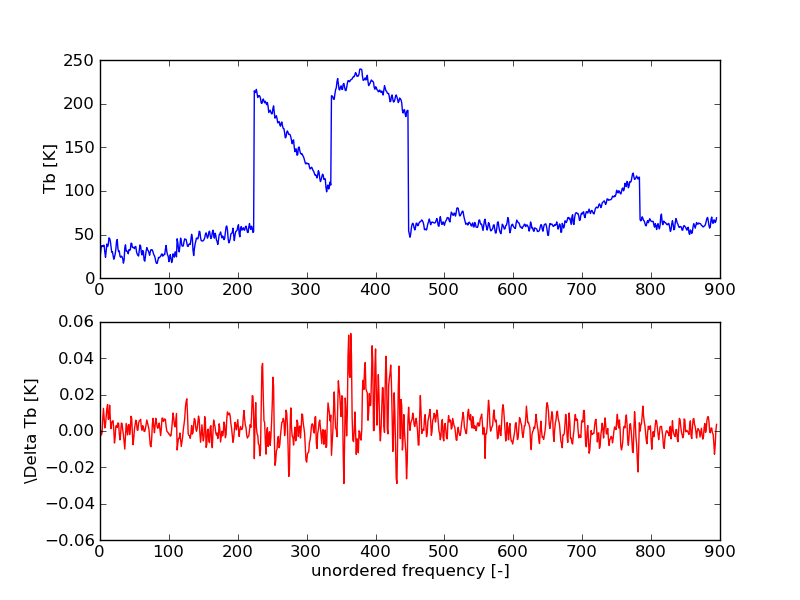
\includegraphics[scale=0.5]{spectrum.png}
\caption{Upper panel: a level1b spectrum from AC1,STW=797932325,
STRAT FM=2 created by the package described in this document,
with a small modification, that is described in text.
Lower panel: difference from the official level1b product
(spectrum found in the file OB1B217F.HDF) }
\label{fig:odin1}
\end{figure}



\subsection{Further development}

\begin{figure}[!t]
\centering
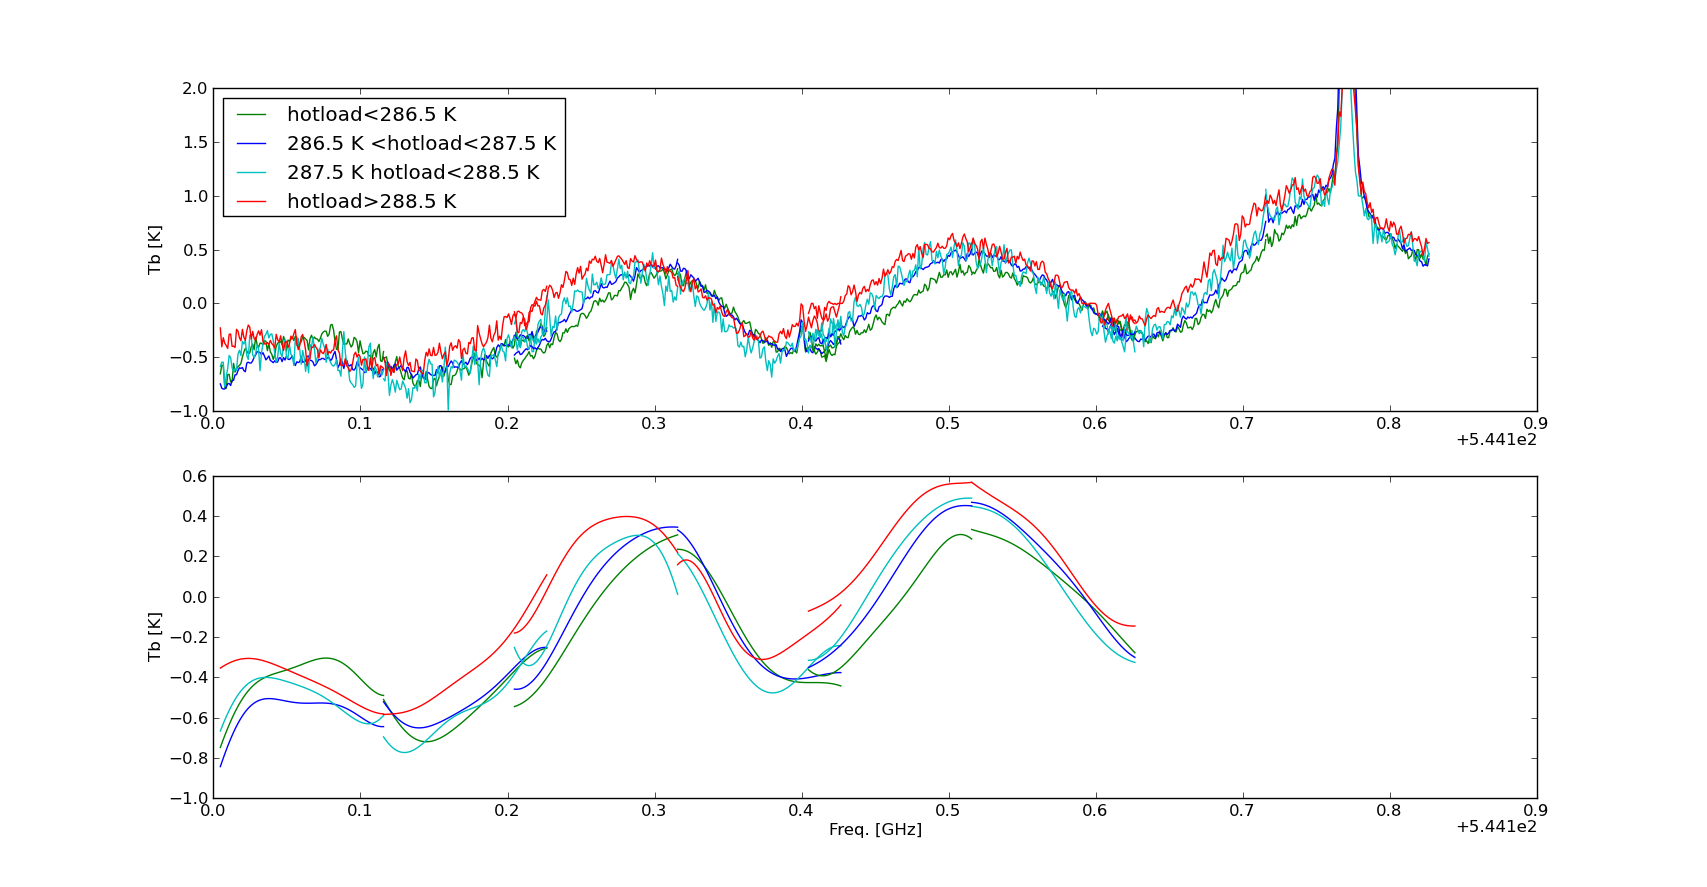
\includegraphics[scale=0.3]{ac1highalt.png}\\
\caption{The upper panel show median of high altitude (60-120 km)
spectra for different temperatures (hotload as a proxy)
for AC1 stratospheric mode 2
from 2009-08-24 to 2009-09-24.
The lower panel shows fits to spectra in the upper panel.}
\label{fig:ac1c}
\end{figure}

We know from earlier studies that both calibrated high and low altitude 
spectra from AC1 and AC2 contains spectral features which not origin
from atmospheric emission. Figure~\ref{fig:ac1c} shows
calibrated high altitude spectra from AC1
using the modified calibration routine. These spectra
should be flat and at a level close 0 K, but they clearly are not flat. 
Figure~\ref{fig:ac1c} also shows that the
spectral pattern has a temperature dependence.
This spectral features should come from that
either the sky signal or the target signal is perturbed. Most likely it comes
from ripple on the sky signal. Regardless where it comes from, it should be
possible to remove this spectral feature in the calibration process.

One way to remove these spectral features would be to:
\begin{itemize}
\item run the calibration routine as it is
\item create a database table with average high and low altitude 
spectra for different temperatures
and for each mode of AC1 and AC2
\item perform a second calibration step of the calibrated spectra
\end{itemize}
 

%level1b\underline{ }importer, which steers the level1b
%calibration, has been written to process data from scans
%that starts in the target orbit.
%The main function of this script starts basically by some
%SQL-queries to find out the start and end stw for the target orbit.
%With this information it is then easy to get all required
%data from the database tables.
%This means that to move away from the orbit based processing
%the main thing to change is the first queries.

%The intensity calibration is performed by a python class
%named Level1b\underline{ }cal that can
%be found in the file level1b\underline{ }importer.py.
%This class has functions as for example:\\
%-- calibrate, that controls the calibration\\
%-- cleanref, that removes spurious cold sky spectrum\\
%-- cleancal, that removes spurious hot load spectrum\\
%-- gain, that calulates tsys spectrum\\
%-- medTsys, that returns a mean Tsys spectrum of all acceptable
%Tsys spectrum\\ 
%calibrate1, that transform signal spectra into an antenna temperature
%scale.
% 
%Laboration with the calibration scheme should not be extremely
%difficult.
  
\section{Required packages and installation}
\subsection{System preparations}
Make sure the following packages are installed in your system.
\begin{verbatim}  
  $> sudo apt-get install libpng12-dev
  $> sudo apt-get install postgresql-server python-setuptools python-dev
  $> sudo apt-get install python-zc.buildout python-numpy libhdf5-serial-dev
  $> sudo apt-get install build-essential postgresql-server-dev-9.1
\end{verbatim}

\subsection{Installation of odincal}

The file buildout.cfg pulls all required packages into a local installation if the required packages with the correct version numbers are installed on the system buildout will use the packages from the system - if they don't exist buildout will build them. The file buildout in Figure \ref{buildout}.

\begin{figure}
\verbatimtabinput{../../buildout_runtime.cfg}
\caption{the file: buildout.cfg}
\label{buildout}
\end{figure}

Create a new directory and copy the buildout.cfg file to it. Run the command buildout2.7 from that directory.


\subsection{Postgresql preparation}
Create a database a database called odin owned by your user. (Tip! use your system username for easier access.)
 
\begin{verbatim}  
  $> sudo -u postgres psql
  psql> create user <your_user_name> login;
  psql> create database odin owner <your_user_name>;
  psql> \q
\end{verbatim}

Install the datamodel.

\begin{verbatim}  
  $> bin/create_datamodel
\end{verbatim}

\subsection{Automatic downloading from PDC}
The rsync tool is used to syncronise the level0 product tree with PDC.
\begin{verbatim}
# kinit must be manually initiation to make this work 'kinit --renewable -l 25h --afslog -f'
47 */12 * * * kinit -R
#13 03 * * * rsync -T /tmp -aLKe "ssh -o 'GSSAPIKeyExchange yes'" --log-file=/home/odinop/odincal/rsync.log --exclude-from=.pdc_excludes donal@pisces.pdc.kth.se:/data/odin/level0/ /misc/pearl/odin/level0/
\end{verbatim}

The --exclude-from refers to a file containing rules for wich directories should be used to syncronisation.

\begin{verbatim}
+ ac1/
+ ac1/*
+ *.ac1
+ ac2/
+ ac2/*
+ *.ac2
+ shk/
+ shk/*
+ *.shk
+ fba/
+ fba/*
+ *.fba
+ att/
+ att/*
+ *.att
- *
\end{verbatim}



\section{Appendix}
\subsubsection*{Matching ac\underline{ }level0 with fba\underline{ }level0}
 One column in the ac\underline{ }level0
table is named sig\underline{ }type and tells if the signal is 
a measurement ('SIG') or reference ('REF').
'REF' can be either a hot load or cold sky signal, and this is
further specified in the fba\underline{ }level0 table,
which contains a column called mech\underline{ }type.
Thus, if sig\underline{ }type is 'REF' one can join the two
tables to find out the type of 'REF' signal.
For example by the sql queries :\\
For ac2 data where the stw match is one to one\\
\begin{verbatim}
select stw, sig_type, mech_type from 
ac_level0 natural join fba_level0 
where sig_type='REF' and backend='AC2';
\end{verbatim}
or for ac1 data where the stw is one stw unit ahead:
\begin{verbatim}
select ac_level0.stw, sig_type,
mech_type from 
ac_level0 join fba_level0 on 
(fba_level0.stw+1=ac_level0.stw) where 
sig_type='REF' and backend='AC1';
\end{verbatim}

\subsubsection*{Example how to extract column data that has Type bytea
or integer[] using python}
To extract data from database tables that have type bytea one must
know the shape and datatype of the data. This information
can be found in the tables in this document. Here is an example
to extract data from the ac\underline{ }level0: 

\begin{verbatim}
import numpy
from pg import DB
class db(DB):
    def __init__(self):
        DB.__init__(self,dbname='odin')

con=db()
query=con.query('''select ssb_fq,cc from ac_level0''')
result=query.dictresult()
cc=numpy.ndarray(shape=(8,96),dtype='float64',
                 buffer=con.unescape_bytea(result[0]['cc']))
ssb_fq=eval(result[0]['ssb_fq'].replace('{','(').replace('}',')'))
\end{verbatim}
\clearpage
\newpage
\subsubsection*{Example how to identify scans}
getscansac1 and getscansac2 are database functions that has been 
created in order to find out scans.
The functions search for data in ac\underline{ }level0
and fba\underline{ }level0 and return stw and start of ac data, 
where start is the stw of the latest calibration measurement. 
The following SQL-queries show how these functions can be used,
and the example also clarifies the meaning of a scan: 
\begin{verbatim}
For AC2

select ac_level0.stw,start,backend,sig_type,mech_type,altitude 
from ac_level0 
natural join fba_level0
natural join attitude_level1
natural join getscansac2() 
where ac_level0.backend='AC2' and start>-1
order by ac_level0.stw;

For AC1

select ac_level0.stw,start,backend,sig_type,mech_type,altitude 
from ac_level0 
natural join attitude_level1
natural join getscansac1() 
join fba_level0 on (fba_level0.stw+1=ac_level0.stw)
where ac_level0.backend='AC1' and start>-1
order by ac_level0.stw;
\end{verbatim}
and can result in someting like:
\begin{verbatim}
    stw     |   start    | backend | sig_type | mech_type | altitude 
------------+------------+---------+----------+-----------+----------
 797831517 | 797831517 | AC1     | SIG      | CAL       |  7744.23
 797831533 | 797831517 | AC1     | REF      | CAL       |  7606.69
 797831549 | 797831517 | AC1     | SIG      | CAL       |     8072
 797831565 | 797831517 | AC1     | REF      | CAL       |   8941.3
 797831581 | 797831517 | AC1     | SIG      | CAL       |   9876.7
 797831597 | 797831517 | AC1     | REF      | CAL       |  10767.3
 797831613 | 797831517 | AC1     | SIG      | SK2       |    11605
 797831629 | 797831517 | AC1     | REF      | SK2       |  12407.1
 797831645 | 797831517 | AC1     | SIG      | SK1       |  13184.4
 797831661 | 797831517 | AC1     | REF      | SK1       |  13950.6
 797831677 | 797831517 | AC1     | SIG      | SK1       |  14704.3
                               .
                                     .
                                     .

 797832604 | 797831517 | AC1     | SIG      | SK1       |    56279
 797832668 | 797831517 | AC1     | REF      | SK1       |  59183.6
 797832732 | 797831517 | AC1     | SIG      | SK1       |  62097.7
 797832796 | 797831517 | AC1     | REF      | SK1       |  64995.9
 797832860 | 797831517 | AC1     | SIG      | SK1       |  67880.1
 797832924 | 797832924 | AC1     | REF      | CAL       |    70724
 797832988 | 797832924 | AC1     | SIG      | CAL       |  69696.1
 797833052 | 797832924 | AC1     | REF      | CAL       |    66386
 797833116 | 797832924 | AC1     | SIG      | CAL       |  63483.4
 797833180 | 797832924 | AC1     | REF      | SK1       |  60660.3
 797833244 | 797832924 | AC1     | SIG      | SK1       |  57801.5 
\end{verbatim}
A scan is here defined as measurements between two hot load (CAL)
measurements. 
These measurements are performed when the scanning turns,
which can be seen in the altitude column.
A scan is identified in the start column, which is the stw
of the hot load measurement in the start of the scan. 
In this examlpe AC1 data with stw 797831517 to 797832860
belongs to scan 797831517. 
\clearpage
\newpage



\clearpage
\newpage

\begin{thebibliography}{1}

\bibitem{notes} M. Ohlberg et al., {\em The Odin satellite
II. Radiometer data processing and calibration},
Astronomy and astrophysics 402, L35--L38, 2003.

\end{thebibliography}

\end{document}




